\vspace{-.2cm}
\section{Discussion}
\myparagraph{Limitations and Future Work} In this work we proposed PH-Reg, a method to reduce the artifact tokens in existing pre-trained vision transformers. We show that PH-Reg can eliminate artifact tokens in ViTs effectively and generate clean dense feature maps, enhancing the performance in downstream dense prediction tasks. This approach relies on test time augmentation to denoise dense feature presentations in the teacher model. While our method generally outperforms DVT on CLIP based models, we sometimes underperform when using the DINOv2 backbone. We believe this is due to the static artifact estimator present in DVT. The assumption of static artifacts holds true for some models (DINOv2), but not for others (CLIP). A potential avenue for additional investigation is how to dynamically determine the artifacts without strong stationary assumptions. 
\myparagraph{Conclusion}
We introduce a novel post-training method PH-Reg, for learning clean dense feature representations in ViTs through an efficient self-distillation framework that does not require additional labeled data. Our approach leverages test-time augmentation to denoise the teacher model, and guide the student model to optimize the dense feature representations.
This enables us to eliminate artifact tokens effectively by integrating learnable registers into existing pretrained models, without the need for training from scratch.
We demonstrate that the distilled ViTs generate fine-grained dense feature maps, enhancing the consistency of feature representations in ViTs. 
We further show that cleaner dense feature maps in ViTs leads to quantifiable improvements on dense prediction tasks. 
Finally, we illustrate that the distilled ViTs can accurately capture meaningful semantic structures in images, as shown by heatmaps generated from CLIP text queries.
We validate our conclusions with extensive evaluations across multiple dense prediction benchmarks.

\begin{figure}[t!]
  \centering
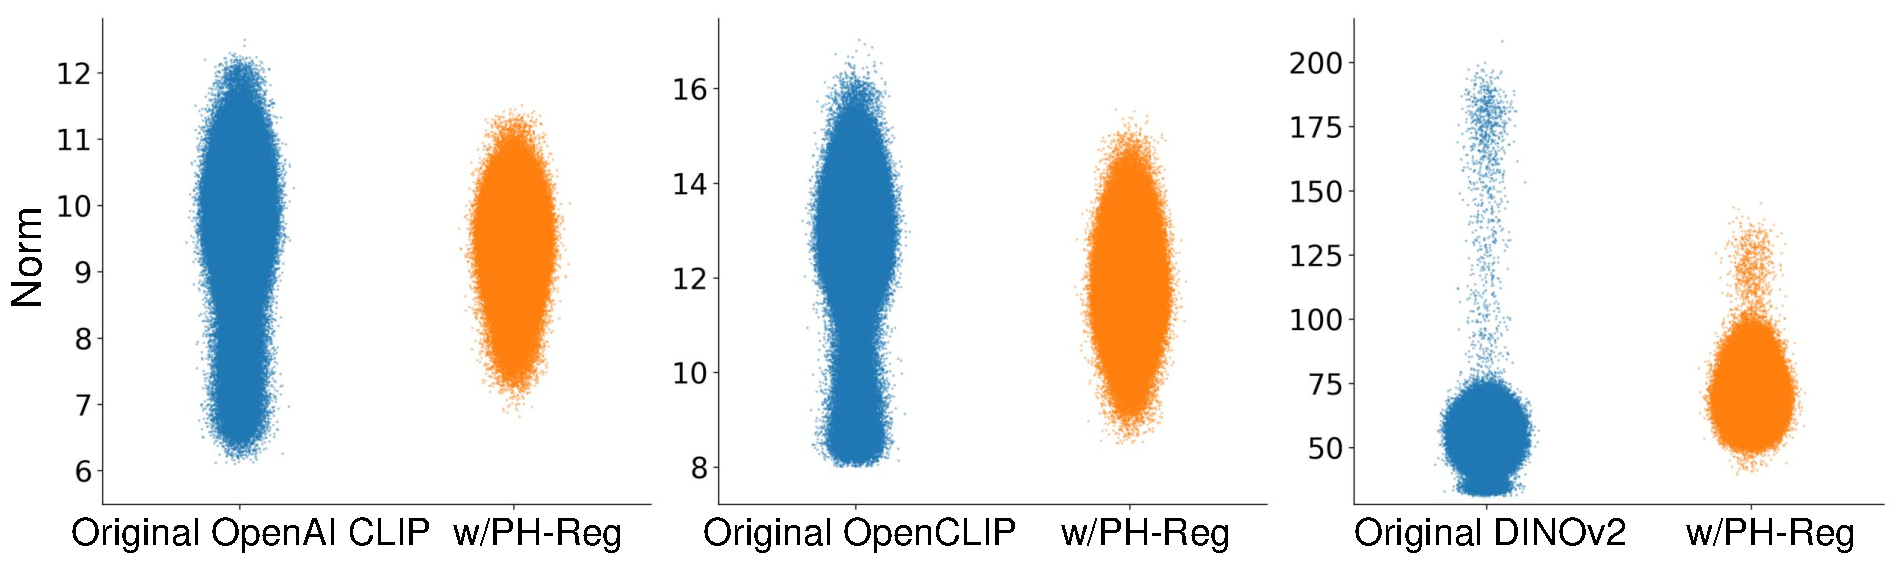
\includegraphics[width=0.85\linewidth]{fig_pdf/visualization_norm_cropped.pdf}
   \vspace{-.1cm}
  \caption{\textbf{Patch Norms.} This figure illustrate norms of patch tokens of different backbones. Our method effectively reduces the variance of token norms and reduces the outliers, regardless if the artifacts are lower/higher norm.}
  \vspace{-.5cm}
  \label{fig:visualization_norm}
\end{figure}